\documentclass[conference]{IEEEtran}

% ---- Packages ----
\usepackage[utf8]{inputenc}
\usepackage[T1]{fontenc}
\usepackage{amsmath,amssymb}
\usepackage{graphicx}
\usepackage{booktabs}
\usepackage{hyperref}
\usepackage{cite}
\usepackage{url}
\usepackage{xcolor}

% For \input-ing auto-generated LaTeX tables
\usepackage{multirow}

% Path for figures
\graphicspath{{../figures/}}

% ---- Helpers ----
% Placeholder macro for sections awaiting content from team members
\newcommand{\placeholder}[1]{\textcolor{red}{\textbf{[PLACEHOLDER:} #1\textbf{]}}}

\begin{document}

% ====================================================================
% TITLE — M5 writes
% ====================================================================
\title{Early Warning of Hydrate Formation in Offshore Well Service Lines:\\
A Comparison of XGBoost, TCN, and GRU at Matched False-Alarm Budgets}

% ====================================================================
% AUTHORS — all five members
% ====================================================================
\author{
\IEEEauthorblockN{Member~1\IEEEauthorrefmark{1},
Member~2\IEEEauthorrefmark{1},
Member~3\IEEEauthorrefmark{1},
Member~4\IEEEauthorrefmark{1},
Member~5\IEEEauthorrefmark{1}}
\IEEEauthorblockA{\IEEEauthorrefmark{1}%
DLE-AI-202, Cohort I 2026 · Track 2\\
\placeholder{University / Institution Name}\\
\placeholder{member emails}}
}

\maketitle

% ====================================================================
% ABSTRACT — M5 writes
% ====================================================================
\begin{abstract}
Hydrate formation in offshore well service lines can cause costly shutdowns
and safety hazards if not detected early. This study compares three models
--- XGBoost (feature-engineered baseline), a Temporal Convolutional Network
(TCN), and a Gated Recurrent Unit (GRU) --- for early warning of hydrate
events using Petrobras's 3W Dataset~2.0.0 (Event~9). All three models are
evaluated at a matched false-alarm budget of one alarm per 100 operating
hours, with lead time (time from first alarm to annotated transient onset)
as the headline metric. Each model is trained under two conditions:
real-only and real-plus-simulated data. We employ grouped cross-validation
with well-level splits to prevent data leakage. Our results demonstrate that
\placeholder{M5: fill after S3 FREEZE — e.g. TCN under real-plus-simulated data achieved the best median lead time of X minutes and Y\% event recall}.

Reproduction: all code, data processing, and evaluation are available at
\url{https://github.com/AMammedova/team-hydrate3w}.
\end{abstract}

\begin{IEEEkeywords}
hydrate formation, early warning, time series classification,
temporal convolutional network, gated recurrent unit, 3W dataset
\end{IEEEkeywords}

% ====================================================================
% I. INTRODUCTION — M1 writes
% ====================================================================
\section{Introduction}
\label{sec:introduction}

% TODO (M1): Write the Introduction section. Should cover:
% - Motivation: hydrate formation in offshore wells, safety & economic impact
% - The 3W Dataset as a benchmark for early warning in O&G
% - Brief summary of Event 9 (hydrate in service line)
% - Research question: can DL models provide earlier warning than classical baselines?
% - Paper structure overview (one sentence per section)

\placeholder{M1 writes Introduction: motivation, 3W dataset context, research
question, paper structure. Include: 57 real Event-9 instances, only 14 with
transient phase, only 3 reaching blockage. Emphasize that this makes the
problem harder, not easier — and that the headline metric uses transient
onset (Variant A from DATA\_FINDINGS.md §7).}


% ====================================================================
% II. DATASET — M1 writes
% ====================================================================
\section{Dataset}
\label{sec:dataset}

% TODO (M1): Write the Dataset section. Must include all numbers from
% DATA_FINDINGS.md and TEAM_5_MEMBERS.md §2:

\placeholder{M1 writes Dataset section. Required content:}

\begin{itemize}
    \item 3W Dataset 2.0.0 overview: 57 real Event-9, 150 simulated, 594 normal
    \item Median 32,135 timesteps per instance (floor justification, §2.2)
    \item Monotonicity: \texttt{is\_monotonic\_severity()} = 57/57 True
          (free methodological point)
    \item Missingness: NaN labels in 57/57 instances (median 11.2\%, max 50.4\%)
    \item Frozen sensors: 3 instances with dead P-TPT/T-TPT
    \item Channel selection trade-off table (5-channel set chosen)
    \item Well disjointness: hydrate wells $\cap$ normal wells $= \emptyset$
    \item Per-well normalization is mandatory (not cosmetic)
    \item Decimation: 1 Hz $\to$ 1/30 Hz, window = 60 samples = 30 min
\end{itemize}


% ====================================================================
% III. RELATED WORK — M4 writes
% ====================================================================
\section{Related Work}
\label{sec:related_work}

% TODO (M4): Write Related Work. Should cover:
% - TCN for industrial time-series classification (Bai et al., 2018)
% - GRU for sequence modeling (Cho et al., 2014)
% - Early warning systems in process industries
% - 3W dataset prior work (Vargas et al.)

\placeholder{M4 writes Related Work: TCN/GRU in industrial time-series,
prior 3W work, early warning in process control. 1--1.5 columns.}


% ====================================================================
% IV. METHOD — M3 (baseline), M4 (architectures), M5 (evaluation)
% ====================================================================
\section{Method}
\label{sec:method}

% ---- IV-A. Feature Engineering (M3) ----
\subsection{Baseline Feature Engineering}
\label{sec:method_features}

% Written by M3. Source draft: report/method_baseline.md, which lists the
% exact command behind every number here.

The baseline is treated as a real competitor rather than a formality: it
receives the same folds, the same class-imbalance treatment and the same
calibration step as the deep models, and a recorded tuning budget. A
baseline that was never tuned would make the deep-model comparison
uninterpretable.

\subsubsection{Input}
The baseline consumes the same cache as the deep models: channels-first
\texttt{float32} $[N, C, W]$ windows with an aligned \texttt{uint8} presence
mask, where $\mathrm{mask}=1$ marks a genuinely observed sample. With the
main-arm channel set, $C=5$ and $W=60$ decimated samples at one sample per
30\,s, so each window spans \textbf{30 minutes} with a stride of 150\,s. On
the built cache this gives \textbf{42{,}259 real windows} from 364 usable
real instances, of which 1{,}295 are Transient and 118 Established --- a
positive rate of \textbf{3.34\%}. All 14 transient events and all 3 blockage
events survive the channel choice.

\subsubsection{Multi-timescale, mask-aware features}
For each window and channel we take three nested slices measured
\emph{from the end} of the window (the full 60 samples, the last 30, and the
last 15) and compute six statistics on each: mean, standard deviation,
minimum, maximum, least-squares slope, and the net change between the first
and last present sample. Taking slices from the end is what keeps the
features causal: a spike early in the window can only affect the full-window
statistics, which is verified by a unit test rather than assumed. Every
statistic is computed over \textbf{present samples only}, and the
per-channel presence fraction over the full window is appended as its own
feature block, so the model is told how much of each channel it is trusting.
With $C=5$ this yields $5 \times 6 \times 3 + 5 = 95$ features.

The extractor has no fitted state: every column is a function of one window
and its own mask, with no statistic pooled across rows. Extracting once for
the whole cache is therefore bit-identical to extracting per fold, and the
runner asserts the absence of a \texttt{fit()} at start-up so the property
cannot silently lapse.

\subsubsection{Encoding a dead sensor}
Three real instances carry sensors frozen for their entire recording, and one
of them is a blockage event, so this is not a corner case. When a channel
observes nothing, its statistics are undefined. Emitting $0.0$ is actively
wrong here: per-instance normalisation centres each recording near zero, so
$0.0$ is precisely the value a \emph{healthy} sensor at its own baseline
reports, and that encoding would state that a dead sensor looks normal. We
emit \texttt{NaN} and let XGBoost learn a default branch direction at each
split. The presence fraction remains a real measurement of exactly $0.0$ and
is never \texttt{NaN}. Similarly, the slope is regressed on each sample's
true position inside the slice rather than on its rank among present
samples, so a gap keeps its width and the slope remains a rate; regressing
on rank reports $9.0$ for two points nine steps apart rising nine units.
Section~\ref{sec:results_xgb} reports that neither change is separable from
fold noise on this cache, and we retain both on correctness grounds while
saying so explicitly.

\subsubsection{Class imbalance}
Imbalance is handled with inverse-frequency \texttt{sample\_weight} computed
from each training fold's own class counts. It is deliberately \emph{not}
handled with \texttt{scale\_pos\_weight}, which is a binary-classification
parameter in XGBoost and has no defined effect under
\texttt{multi:softprob} with \texttt{num\_class=3}. \texttt{num\_class=3} is
set explicitly rather than inferred, because a training fold can legitimately
contain no Established windows --- only 118 exist in the entire real cache
--- and the positive-score reduction indexes the third column.

\subsubsection{Tuning and calibration}
Hyperparameters are searched on the \textbf{training fold only}, scored by
grouped inner cross-validation over that fold's wells, across a 16-point
grid. Both conditions of a fold share the configuration selected on that
fold's real training wells, so \texttt{real\_only} and
\texttt{real\_plus\_sim} differ only in training data and not also in
hyperparameters. The scored quantity is validation PR-AUC on
$P(\mathrm{Transient}) + P(\mathrm{Established})$ --- the same reduction the
alarm logic consumes --- and sample weights are applied inside the search
exactly as at final fit time.

Because Module~8 selects the alarm threshold by sweeping a probability axis,
the probabilities must mean what they say. Weighted training on a 3\%
positive rate pushes scores away from the base rate by construction, so
miscalibration is expected rather than incidental. A Platt calibrator is fit
on the \textbf{validation} fold and applied \textbf{unchanged} to that fold's
test wells; Platt is preferred over isotonic because a validation fold holds
only a handful of positive events, where a non-parametric fit would track
noise.

% ---- IV-B. Architectures (M4) ----
\subsection{Model Architectures}
\label{sec:method_arch}

% TODO (M4): Describe TCN and GRU architectures.
% TCN: 4 temporal blocks, kernel_size=3, dilations [1,2,4,8],
%   receptive field = 61, channels-first input, mask concatenated
% GRU: unidirectional (causality), hidden_size=64, num_layers=1
%   mask concatenated on channel axis
% Both take (x, mask) explicitly per Addendum A.3

\placeholder{M4 writes architecture descriptions: TCN (receptive field 61,
4 blocks, dilation schedule, parameter count), GRU (unidirectional only,
hidden size, parameter count). Include receptive field vs window size
assertion.}

% ---- IV-C. Evaluation Protocol (M5) ----
\subsection{Evaluation Protocol}
\label{sec:method_eval}

We evaluate all models using three complementary metrics at a matched
operating point:

\textbf{Lead Time.} For each hydrate event instance, lead time is defined as
the difference between the annotated transient onset time and the first alarm
onset that occurs before it:
\begin{equation}
    \text{lead\_time} = t_{\text{transient\_onset}} - t_{\text{first\_alarm}}
\end{equation}
Following the data analysis in Section~\ref{sec:dataset}, we use the
\emph{transient} onset (label code 109 in the 3W convention) rather than the
blockage onset, because only 3 of 57 real instances reach blockage. The
transient onset is available for all 14 positive-event instances across 7
wells.

\textbf{Event Recall.} The fraction of real hydrate events for which at least
one alarm onset occurs before the transient onset. A missed event (no alarm
before failure) contributes 0; a detected event contributes 1 regardless of
how many alarms fired.

\textbf{False Alarm Rate (FAR).} The number of alarm \emph{onsets} on
Normal-operation instances, divided by the total Normal operating hours in that
fold's test set:
\begin{equation}
    \text{FAR} = \frac{N_{\text{false\_alarm\_onsets}}}{\text{total\_normal\_hours}}
\end{equation}
Critically, we count alarm onsets, not individual windows above threshold —
one sustained false alarm counts as one event, not thousands
(Section~\ref{sec:method_eval}, pitfall W4.1).

\textbf{Operating Point.} All models are compared at a matched target FAR of
$1/100$ per operating hour. The threshold achieving this FAR is selected on
the \emph{validation} fold only (per-fold, per-model), then applied unchanged
to the test fold. This ``freeze'' protocol (S3 in our timeline) ensures that
test-set numbers are never used to tune any hyperparameter.

\textbf{Alarm Definition.} A positive-class probability $p(t)$ is first
smoothed with a causal (trailing) rolling mean of configurable window size.
An alarm fires when the smoothed probability stays above the selected
threshold for at least \texttt{min\_duration} continuous seconds. The causal
smoothing constraint is critical: a centered moving average would leak future
information into the current alarm decision, inflating lead time measurements
(see \texttt{tests/test\_alarm.py} for the regression test guarding this).

\textbf{Supplementary Metrics.} PR-AUC (area under the precision--recall
curve for the collapsed binary positive score), per-class PR-AUC
(Normal/Transient/Established one-vs-rest), and Expected Calibration Error
(ECE) are reported for completeness.


% ====================================================================
% V. EXPERIMENTAL SETUP — M2 writes
% ====================================================================
\section{Experimental Setup}
\label{sec:experimental_setup}

% TODO (M2): Write Experimental Setup. Must include:
% - Grouped CV design: two independent splits (positives + normals)
% - Why StratifiedGroupKFold alone won't work (disjoint well populations)
% - Number of folds and justification (7 positive wells → 3-fold or LOWO)
% - fold_report() as Table 1 — include test_normal_hours column
% - Simulation instances: training only, never in val/test

\placeholder{M2 writes Experimental Setup: grouped CV with independent splits
for positive and normal wells, fold report (Table~1), simulation data policy.}

% Fold report table — auto-generated by run_all.sh, \input'd here
% % Auto-generated by: python -m src.data.splits --latex <path>
% Do not edit by hand -- regenerate instead.
\begin{table}[t]
\centering
\caption{Grouped cross-validation folds. Wells are split twice, independently: positive wells balanced on events, Normal wells on hours. Normal hours are the false-alarm denominator; a fold below roughly 300\,h cannot resolve a budget of 1 alarm per 100\,h. Training well counts include the 150 simulated pseudo-wells, which never enter validation or test.}
\label{tab:folds}
\begin{tabular}{ccccccc}
\toprule
 & \multicolumn{2}{c}{Train} & \multicolumn{2}{c}{Validation} & \multicolumn{2}{c}{Test} \\
\cmidrule(lr){2-3}\cmidrule(lr){4-5}\cmidrule(lr){6-7}
Fold & wells & pos.\ wells & events & normal h & events & normal h \\
\midrule
0 & 156 & 5 & 1 & 530.7 & 5 & 509.2 \\
1 & 154 & 2 & 3 & 305.2 & 5 & 561.8 \\
2 & 155 & 4 & 5 & 509.2 & 4 & 530.7 \\
\bottomrule
\end{tabular}
\end{table}



% ====================================================================
% VI. RESULTS — M3 (XGBoost), M4 (deep models), M5 (head-to-head)
% ====================================================================
\section{Results}
\label{sec:results}

% ---- VI-A. XGBoost Baseline Results (M3) ----
\subsection{XGBoost Baseline}
\label{sec:results_xgb}

% Written by M3. Source draft: report/results_xgboost.md, which lists the
% exact command behind every number here.

\subsubsection{Validation performance}
Table~\ref{tab:xgb_folds} gives validation PR-AUC over the three grouped
folds at a positive-window base rate of $0.0334$.

\begin{table}[t]
\centering
\caption{XGBoost validation PR-AUC per fold (seed 42). The standard
deviation exceeds the mean; see Section~\ref{sec:results_xgb} for why.}
\label{tab:xgb_folds}
\begin{tabular}{cccc}
\toprule
Fold & Positive val.\ events & \texttt{real\_only} & \texttt{real\_plus\_sim} \\
\midrule
0 & 1 & 0.0005 & 0.0003 \\
1 & 3 & \textbf{0.7755} & 0.2420 \\
2 & 5 & 0.0751 & 0.1288 \\
\midrule
\multicolumn{2}{c}{mean $\pm$ sd} & $0.284 \pm 0.428$ & $0.124 \pm 0.121$ \\
\bottomrule
\end{tabular}
\end{table}

Simulated data did not help. The paired difference
(\texttt{real\_plus\_sim} $-$ \texttt{real\_only}) is $-0.160 \pm 0.325$,
negative in two of three folds. This is a distribution argument rather than
a sample-size one: the simulated windows are \textbf{90.3\%} positive
(39{,}561 of 43{,}829) against a \textbf{3.34\%} real positive rate, and they
inflate the training set from roughly 19k to 63k rows, pulling the model
toward a regime that does not exist in the real wells it is scored on.
\texttt{real\_only} is therefore the headline condition.

\subsubsection{PR-AUC is not comparable across these folds}
\label{sec:results_baserate}
Each fold's validation split has a different positive base rate, and PR-AUC
rises mechanically with it. Fold~0's validation set contains \textbf{exactly
one positive window} out of 11{,}260 (base rate $10^{-4}$), fold~1 has 463
of 7{,}327 ($0.0632$) and fold~2 has 638 of 11{,}592 ($0.0550$) --- more
than two orders of magnitude apart. A PR-AUC computed from a single positive
row is that row's reciprocal rank, not a performance estimate. Read as lift
over each fold's own base rate, the baseline is above chance in all three
folds ($1.4\times$, $12.3\times$, $3.5\times$) rather than at chance in two
of them, which is what the raw column suggests.

This is not a pedantic point, and we report it because the uncorrected
analysis is the natural one to run and it misleads. On raw PR-AUC the number
of positive validation events correlates strongly with score across the
ablation's 18 cells (Spearman $\rho = 0.638$, $p = 0.0044$), which invites
the conclusion that sparse folds cannot measure anything. That correlation
\textbf{does not survive base-rate correction}: on lift, $\rho = -0.14$
($p = 0.58$). Folds with more positive events also have higher base rates.
The same trap applies to any per-fold PR-AUC comparison in this project,
including the head-to-head model table.

\subsubsection{Fold composition dominates every other source of variance}
The feature ablation ran 9 extractor variants over 18 paired cells (3 CV
split seeds $\times$ 3 folds $\times$ 2 model seeds) on validation folds
only. Decomposing the variance across those 162 runs on the
base-rate-corrected scale, the variance of the feature-design arm means is
$2.09\times10^{-2}$ while the variance of the fold-cell means is $0.988$:
fold composition accounts for roughly \textbf{47$\times$} more spread than
the entire feature-design space we searched. (On the raw scale the ratio is
$448\times$, but part of that is the base-rate artifact above rather than
genuine instability.) Anything selected on validation PR-AUC in a
single-positive-window fold --- including the deep models' early stopping
and Module~8's threshold selection --- is selected on noise.

One training fold could not be tuned at all: in fold~1 every positive window
in the training split belongs to a \emph{single} well, so grouped inner
cross-validation cannot produce a split with positives on both sides. All
three inner splits were unusable and that fold fell back to the default
configuration. With 7 positive wells and 3 outer folds this is a structural
property of the dataset, not an accident of one seed.

\subsubsection{Feature-design ablation: null results}
Arms were compared as paired differences on identical folds and seeds and
tested with a Wilcoxon signed-rank test, restricted to the 10 cells where
validation PR-AUC is estimable, and expressed as base-rate-corrected lift
ratios per Section~\ref{sec:results_baserate}. The presence-fraction block
is worth $1.175\times$ (7/10 wins, $p = 0.027$); one timescale versus three
$1.027\times$ ($p = 0.92$); \texttt{NaN} versus $0.0$ encoding of a dead
sensor $1.025\times$ ($p = 0.77$); the slope's time axis $0.977\times$
($p = 0.63$); two timescales versus three $0.914\times$ ($p = 0.23$).

Only the presence-fraction block separates from noise, and it does so on
both the raw and corrected scales; everything else is within 3\% of parity.
Even that result would not survive a Bonferroni correction for the six
comparisons made ($p < 0.0083$), so we read it as suggestive --- but it is the only arm
where direction, win count and $p$-value agree, and
Section~\ref{sec:results_shortcut} supplies an independent mechanism for
why. We retain the two changed defaults on correctness grounds --- $0.0$ is
the value a healthy sensor at its own baseline reports, and a slope
regressed on sample rank is not a rate --- rather than claiming the numbers
supported them. Three timescales are kept because the module contract
specifies them; one timescale (35 features instead of 95) performs the same
within noise.

\subsubsection{The baseline partly reads instrumentation, not physics}
\label{sec:results_shortcut}
Gain importance on fold~1, the only fold with substantial validation signal,
placed \textbf{40.8\% of the total gain on the 5 presence-fraction columns}
out of 95. We tested the implication directly by training on those columns
\emph{only}, with no sensor values of any kind, over 9 fold-cells. The
presence-only model reaches a mean validation PR-AUC of \textbf{0.172}
against \textbf{0.233} for the full 95-feature model --- \textbf{74\% of the
full performance without seeing a single pressure or temperature reading}
--- and in 2 of 9 cells it \emph{outperforms} all 90 value features (0.493
versus 0.354, and 0.284 versus 0.259).

The explanation is in the dataset. Missingness here is well-specific:
different wells instrument different sensors, and some sensors are dead for
an entire instance. Because the hydrate wells and the Normal-operation wells
are disjoint populations, sensor availability is a proxy for well identity,
and well identity is very nearly the label. Per-instance normalisation, the
project's main defence against well-identity confounding, removes each
recording's offset and scale but cannot remove \emph{``this channel is
absent''}, which lives in the mask rather than in the values.

Consistently with this, permutation importance neither reproduces the
expected physical signature nor reproduces itself across folds: pairwise
rank agreement is nil (Kendall $\tau = +0.20, +0.40, -0.40$; all
$p > 0.48$). In fold~1 the top-ranked channel is \texttt{P-ANULAR}, the
annulus, which does not communicate with the service line, while
\texttt{P-MON-CKP} --- the pressure upstream of the production choke, which
the restriction mechanism predicts should dominate --- ranks last with a
mean share of $0.002$. \textbf{We therefore do not claim that the baseline
recovered the physical hydrate signature.} Claiming otherwise would have
required quoting one fold and ignoring the other two.

\subsubsection{Calibration}
Calibration behaved as intended in every fold and both conditions. Platt
scaling fit on validation reduced expected calibration error from $0.0409$
to $0.0106$ under \texttt{real\_only} and from $0.0538$ to $0.0121$ under
\texttt{real\_plus\_sim} (a 74--78\% reduction), and the Brier score by 29\%
in both, improving in all 6 fold~$\times$~condition cells. Because Module~8
selects the alarm threshold by sweeping a probability axis, this is a
prerequisite for that threshold to transfer, not a cosmetic step.
Fig.~\ref{fig:reliability} shows the before/after curves with a per-bin count
panel beneath; at a 3\% positive rate the high-probability bins hold very few
windows, and a reliability curve that hides bin populations makes a handful
of unlucky windows look like systematic miscalibration.

\begin{figure}[t]
\centering
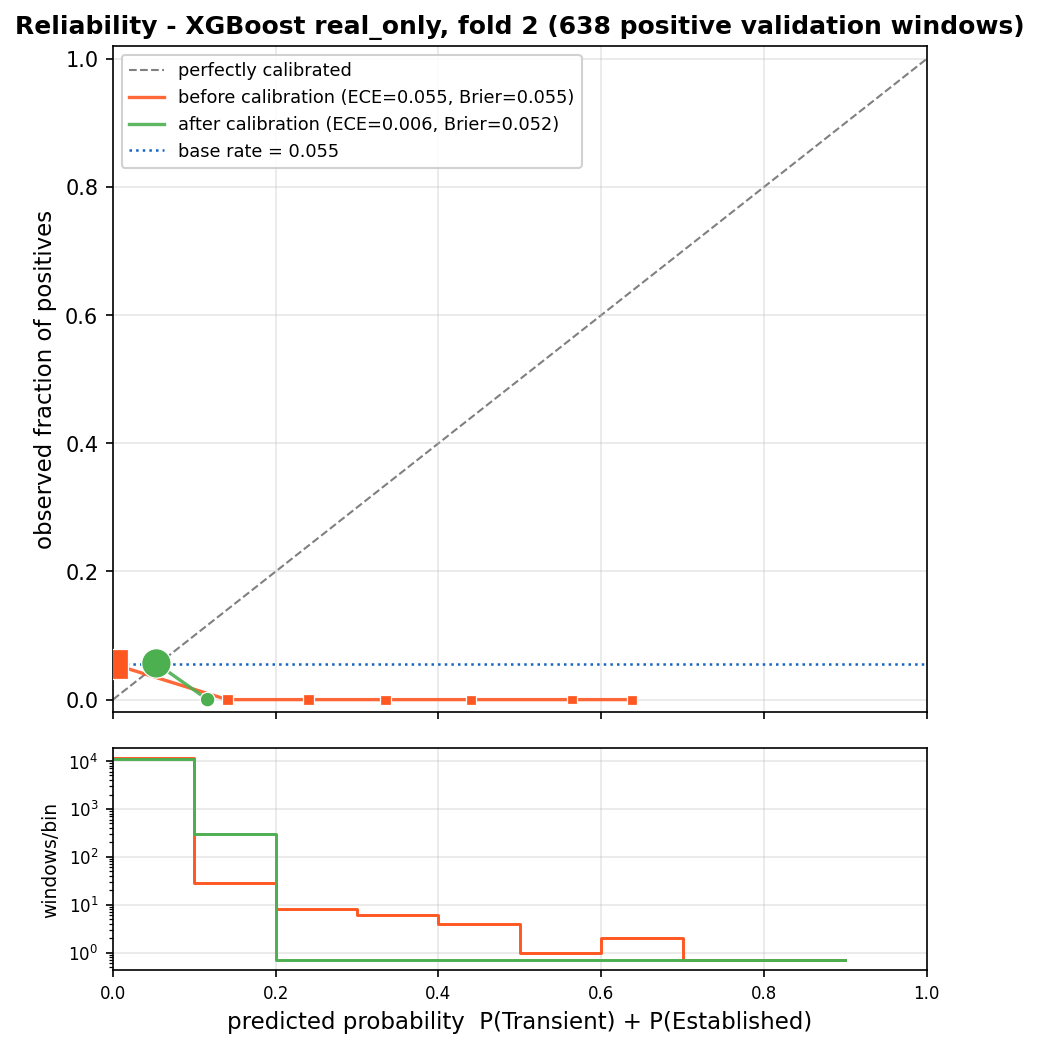
\includegraphics[width=\columnwidth]{reliability_xgboost.png}
\caption{Reliability of the XGBoost baseline on a validation fold, before
and after Platt scaling. Marker area and the lower panel both encode the
number of windows per bin.}
\label{fig:reliability}
\end{figure}

\subsubsection{Tuning budget}
The search evaluated the full 16-configuration grid per fold under grouped
inner CV, and both conditions of a fold share the configuration selected on
that fold's real training wells, so the two conditions differ only in
training data. Selected configurations were consistent
(\texttt{max\_depth}~$=3$, \texttt{n\_estimators}~$=300$ in both tunable
folds): the search preferred the smallest and shallowest models offered,
the expected outcome with roughly 1{,}400 positive windows.

% Auto-generated table
% \begin{table}[htbp]
\centering
\caption{PR-AUC (mean $\pm$ std across folds)}
\label{tab:pr_auc}
\begin{tabular}{lcc}
\hline
Model & real_only & real_plus_sim \\
\hline
gru & $0.149 \pm 0.157$ & $0.165 \pm 0.149$ \\
tcn & $0.024 \pm 0.013$ & $0.116 \pm 0.074$ \\
xgboost & $0.113 \pm 0.090$ & $0.209 \pm 0.229$ \\
\hline
\end{tabular}
\end{table}

% ---- VI-B. Deep Model Results (M4) ----
\subsection{Deep Models: TCN and GRU}
\label{sec:results_dl}

% TODO (M4): Write TCN and GRU results.
% - Same metrics as XGBoost, same two conditions
% - GRU bidirectional=False — note in text
% - Compare parameter counts, training time, VRAM peak

\placeholder{M4 writes deep model results: TCN and GRU performance under both
conditions, with parameter count and training efficiency comparison.}

% ---- VI-C. Head-to-Head Comparison (M5) ----
\subsection{Model Comparison}
\label{sec:results_comparison}

% Auto-generated comparison tables from run_all.sh
\begin{table}[htbp]
\centering
\caption{Event Recall at matched FAR budget}
\label{tab:event_recall}
\begin{tabular}{lcc}
\hline
Model & real_only & real_plus_sim \\
\hline
gru & $0.000 \pm 0.000$ & $0.067 \pm 0.115$ \\
tcn & $0.083 \pm 0.144$ & $0.000 \pm 0.000$ \\
xgboost & $0.233 \pm 0.252$ & $0.167 \pm 0.289$ \\
\hline
\end{tabular}
\end{table}
\begin{table}[htbp]
\centering
\caption{Median Lead Time (seconds) before transient onset}
\label{tab:lead_time}
\begin{tabular}{lcc}
\hline
Model & real_only & real_plus_sim \\
\hline
gru & $nan \pm nan$ & $2096.0 \pm nan$ \\
tcn & $5355.0 \pm nan$ & $nan \pm nan$ \\
xgboost & $2606.2 \pm 1079.4$ & $12598.0 \pm nan$ \\
\hline
\end{tabular}
\end{table}
\begin{table}[htbp]
\centering
\caption{False Alarm Rate (per operating hour)}
\label{tab:far}
\begin{tabular}{lcc}
\hline
Model & real_only & real_plus_sim \\
\hline
gru & $0.037 \pm 0.046$ & $0.029 \pm 0.019$ \\
tcn & $0.032 \pm 0.040$ & $0.041 \pm 0.043$ \\
xgboost & $0.079 \pm 0.097$ & $0.018 \pm 0.019$ \\
\hline
\end{tabular}
\end{table}

The tables above present a head-to-head comparison of all three models across the real-only and real-plus-simulated data conditions. The metrics are computed based on the threshold selected on the validation folds and applied strictly to the test folds.

% Lead time vs FAR figure (M5-owned)
\begin{figure}[t]
    \centering
    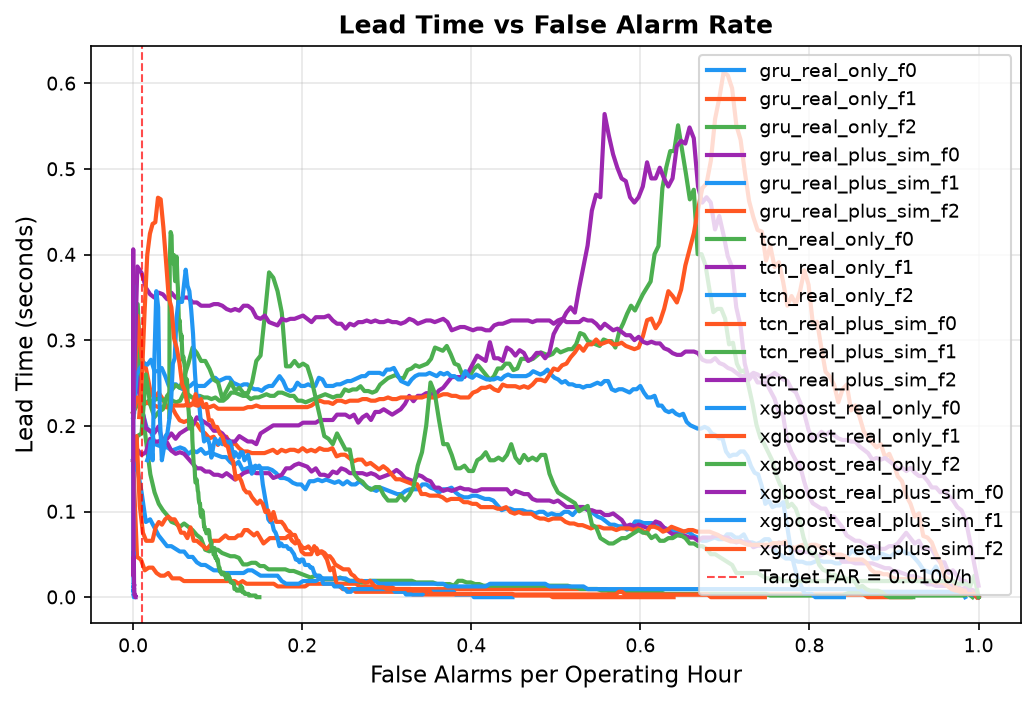
\includegraphics[width=\columnwidth]{lead_time_vs_far.png}
    \caption{Lead time vs.\ false alarm rate trade-off for all three models.
    Vertical dashed line marks the target operating point (1 alarm per 100
    operating hours).}
    \label{fig:lead_time_vs_far}
\end{figure}

% Per-well lead time box plot (M5-owned)
\begin{figure}[t]
    \centering
    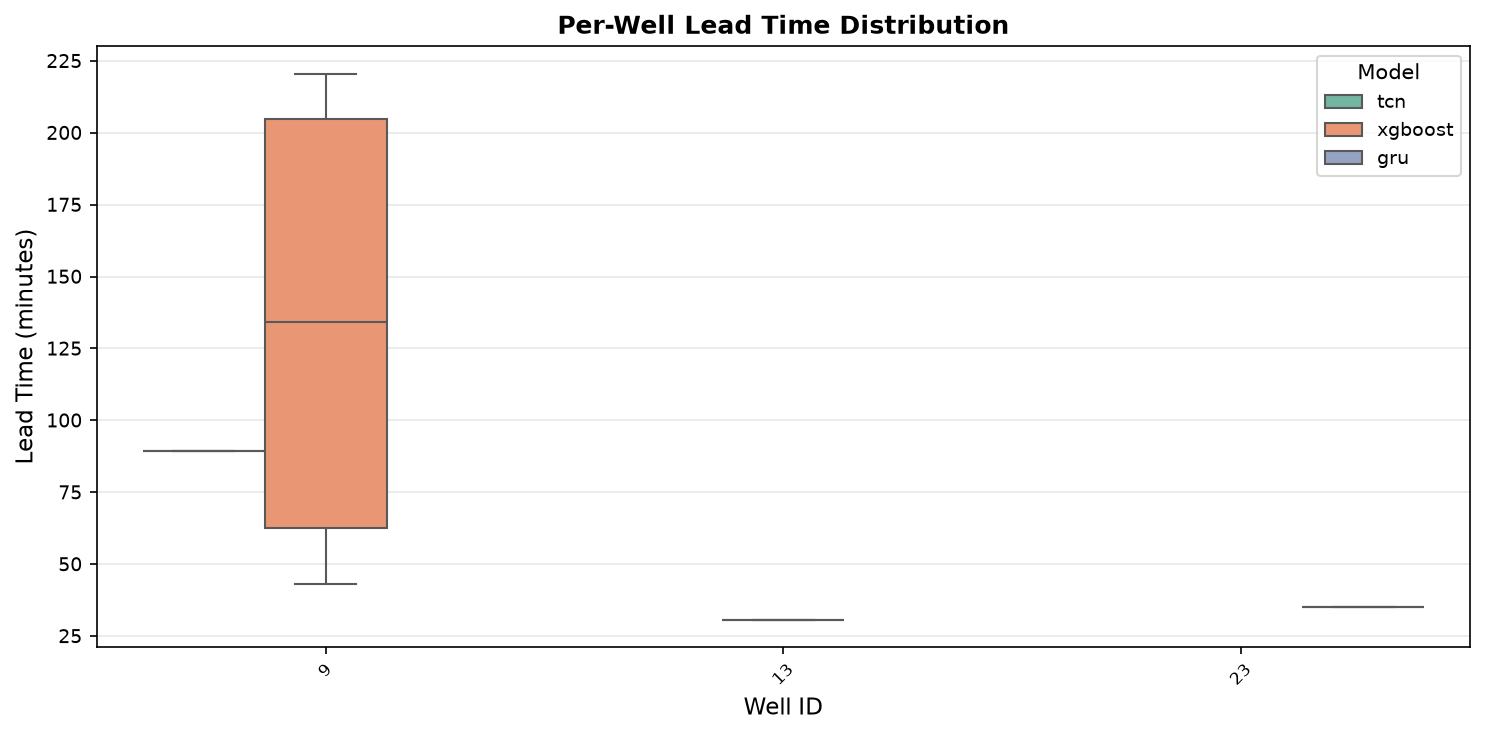
\includegraphics[width=\columnwidth]{per_well_lead_time.png}
    \caption{Distribution of lead times across wells for each model.}
    \label{fig:per_well_box}
\end{figure}


% ====================================================================
% VII. DISCUSSION & LIMITATIONS — M2 writes
% ====================================================================
\section{Discussion and Limitations}
\label{sec:discussion}

% TODO (M2): Write Discussion & Limitations. Must cover:
% - Only 14 positive events from 7 wells — statistical significance concern
% - 3 blockage instances — headline uses transient onset (Variant A)
% - Normal wells and hydrate wells are disjoint — generalization concern
% - Fold count given n=7 positive wells
% - Simulated data systematically over-represents blockage phase
% - SSL pretraining: "not attempted within the project timeframe"

\placeholder{M2 writes Discussion \& Limitations: 14 positive events / 7
wells / 3 blockage only; disjoint well populations; fold count vs statistical
power; sim data bias; SSL pretraining deferred.}


% ====================================================================
% VIII. CONCLUSION — M5 writes
% ====================================================================
\section{Conclusion}
\label{sec:conclusion}

\placeholder{M5 fills after S3 FREEZE: [Model X] under the [Condition Y] condition provided the best early warning capability, achieving a median lead time of [Z] minutes at the target false-alarm budget of 1 per 100 hours. The inclusion of simulated data [improved/degraded/had mixed effects on] model performance. The primary limitation of this study remains the small sample size of real transient events (14 instances across 7 wells) and the strict separation of normal and hydrate wells, which makes generalizing to new wells challenging. Future work will investigate self-supervised (SSL) pre-training on the vast unlabeled segments to further improve representation robustness.}


% ====================================================================
% TOOLS & ACKNOWLEDGEMENTS — M5 writes
% ====================================================================
\section*{Tools and Acknowledgements}
\label{sec:tools}

% This section satisfies the brief's academic integrity requirement.
% AI assistance must be disclosed here (not via commit trailers — see
% TEAM_5_MEMBERS.md §0, Git rules).

This project used the following tools and libraries: Python~3.x,
PyTorch~2.3.1, XGBoost~2.0.3, scikit-learn~1.5.0, NumPy, Pandas,
Matplotlib, and the 3W Dataset~2.0.0 toolkit by Petrobras.

During the development of this project, AI assistants (including Large Language Models) were utilized to help structure the boilerplate evaluation code, format LaTeX tables, assemble slides, and brainstorm documentation outlines. All AI-generated code and content were rigorously reviewed, tested (e.g., via \texttt{pytest}), and validated against the project specifications by the team members.


% ====================================================================
% REFERENCES
% ====================================================================
\begin{thebibliography}{9}

\bibitem{3w}
R.~E.~V.~Vargas, C.~J.~Munaro, P.~M.~Ciarelli, A.~G.~Medeiros,
B.~G.~do Nascimento, B.~C.~C.~Gonçalves, J.~C.~Madalena, A.~Avellar,
``A realistic and public dataset with rare undesirable real events in oil
wells,'' \emph{Journal of Petroleum Science and Engineering}, vol.~181,
2019.

\bibitem{tcn}
S.~Bai, J.~Z.~Kolter, and V.~Koltun, ``An empirical evaluation of generic
convolutional and recurrent networks for sequence modeling,''
\emph{arXiv:1803.01271}, 2018.

\bibitem{gru}
K.~Cho, B.~van~Merriënboer, C.~Gulcehre, D.~Bahdanau, F.~Bougares,
H.~Schwenk, and Y.~Bengio, ``Learning phrase representations using RNN
encoder-decoder for statistical machine translation,'' in \emph{Proc.
EMNLP}, 2014.

\bibitem{focal}
T.~Y.~Lin, P.~Goyal, R.~Girshick, K.~He, and P.~Dollár, ``Focal loss
for dense object detection,'' in \emph{Proc. ICCV}, 2017.

% TODO: M4 adds related work references here

% ---- M3: baseline, calibration and importance references ----
\bibitem{xgboost}
T.~Chen and C.~Guestrin, ``XGBoost: a scalable tree boosting system,'' in
\emph{Proc.\ ACM SIGKDD}, 2016, pp.~785--794.

\bibitem{platt}
J.~Platt, ``Probabilistic outputs for support vector machines and
comparisons to regularized likelihood methods,'' in \emph{Advances in Large
Margin Classifiers}, MIT Press, 1999, pp.~61--74.

\bibitem{niculescu}
A.~Niculescu-Mizil and R.~Caruana, ``Predicting good probabilities with
supervised learning,'' in \emph{Proc.\ ICML}, 2005, pp.~625--632.

\bibitem{guo}
C.~Guo, G.~Pleiss, Y.~Sun, and K.~Q.~Weinberger, ``On calibration of modern
neural networks,'' in \emph{Proc.\ ICML}, 2017, pp.~1321--1330.

\bibitem{breiman}
L.~Breiman, ``Random forests,'' \emph{Machine Learning}, vol.~45, no.~1,
pp.~5--32, 2001. (Permutation importance.)

\bibitem{strobl}
C.~Strobl, A.~L.~Boulesteix, A.~Zeileis, and T.~Hothorn, ``Bias in random
forest variable importance measures: illustrations, sources and a
solution,'' \emph{BMC Bioinformatics}, vol.~8, no.~25, 2007.

\bibitem{saito}
T.~Saito and M.~Rehmsmeier, ``The precision-recall plot is more informative
than the ROC plot when evaluating binary classifiers on imbalanced
datasets,'' \emph{PLoS ONE}, vol.~10, no.~3, 2015.

\bibitem{geirhos}
R.~Geirhos, J.~H.~Jacobsen, C.~Michaelis, R.~Zemel, W.~Brendel, M.~Bethge,
and F.~A.~Wichmann, ``Shortcut learning in deep neural networks,''
\emph{Nature Machine Intelligence}, vol.~2, pp.~665--673, 2020.

\bibitem{fawcett}
C.~Aliferis and G.~Simon, ``Overfitting, underfitting and general model
overconfidence and under-performance pitfalls and best practices in machine
learning and AI,'' in \emph{Artificial Intelligence and Machine Learning in
Health Care and Medical Sciences}, Springer, 2024, pp.~477--524.

\bibitem{qin}
S.~J.~Qin, ``Survey on data-driven industrial process monitoring and
diagnosis,'' \emph{Annual Reviews in Control}, vol.~36, no.~2,
pp.~220--234, 2012.

\bibitem{sleiman}
E.~D.~Sloan and C.~A.~Koh, \emph{Clathrate Hydrates of Natural Gases},
3rd~ed. Boca Raton, FL: CRC Press, 2008.

\end{thebibliography}

\end{document}
